\section{Possibility Result} \label{sec:result}

In this section, we present our main possibility result for achieving time-delayed-fairness assuming the network is synchronous and ignore communication and computation cost. 


\paragraph{Notations} Throughout the paper, when we assume the network is synchronous, we use $\synctime$ to denote the maximum dalay for a transaction to be disseminated to all honest nodes after it is sent by a honest node. We use $\thtime$ to denote the time-delay parameter in our time-delayed-fairness definition. We use $n$ to denote the total number of nodes and $h$ to denote the ratio of honest nodes. Use $\allset$, $\hset$ and $\aset$ to denote the set of all nodes, the set of honest nodes, and the set of adversary nodes. We use $\varphi$ to denote the threshold ratio for a transaction $\tx$ to be considered as received before another transaction $\tx'$. 

\paragraph{Synchrony assumption} In this section, we assume the network is synchronous with parameter $\synctime$.  

\paragraph{Adversary model} We assume a static Byzantine adversary that can corrupt up to $n(1-h)$ nodes, where $h>2/3$. The adversary can coordinate the corrupted nodes to deviate from the protocol in any way. The adversary can also delay or reorder messages sent by honest nodes, but cannot forge messages. 

\paragraph{Notation - Timestamp} For a node $i$, denote its timestamp for a transaction $\tx$ as $\ts_i(\tx)$. In our setting, guaranteed by Byzantine broadcast, if an honest node confirms a valid timestamp $\ts_i(\tx)$ by node $i$, all other nodes confirm the same timestamp $\ts_i(\tx)$ for node $i$ receiving $\tx$. If node $i$ does not broadcast its timestamp for $\tx$, it is considered missing, all honest nodes infer that node $i$ will receive $\tx$ in the future if $\tx$ is ever disseminated. 

\paragraph{Notation - Precede relation} For two transactions $\tx$ and $\tx'$, the set of $n$ nodes $\allset$ participating in the transaction ordering scheme, denote $\nset_{\thtime}(\tx, \tx')$ as the set of nodes that receive $\tx$ at least $\thtime$ before $\tx'$, i.e., $\nset_{\thtime}(\tx, \tx') = \{i\in \allset: \ts_i(\tx) + \thtime\le \ts_i(\tx')\}$. We say there is a ($\thtime, \varphi$)-precede relation between $\tx$ and $\tx'$, denoted as $\tx \prec_{\thtime, \varphi} \tx'$, if $|\nset_{\thtime}(\tx, \tx')| \ge n\varphi$. When the context is clear, we omit the subscripts and simply write $\nset(\tx, \tx')$ and $\tx \prec \tx'$. Using the above notation, time-delayed-fairness requires that for any pair of two transactions $\tx$ and $\tx'$ such that $\tx\prec \tx'$,  $\tx$ should be delivered before $\tx'$. 

\paragraph{Protocol Design} Transaction ordering protocols in this section do not consider communication and computation cost, in order to achieve time-delayed-fairness with the tightest parameters possible. For every node, upon receiving a transaction, it records the time of receiving the transaction and runs a Byzantine broadcast protocol for the transaction along with its timestamp. Under the assumption that the network is $\synctime$-synchronous and more than $2/3$ nodes are honest, Byzantine broadcast protocols terminate in bounded time when the broadcaster is honest.  By Byzantine broadcast, if an honest node $i$ confirms a transaction $\tx$ with timestamp $t$ from a node $j$, all other honest nodes also confirm that node $j$ receive $\tx$ at time $t$. Therefore, all honest nodes have the same view of the time when each node receives a transaction. Our trsanction ordering mechanism outputs an order of transactions based on the view of timestamps of all nodes and existing part of blockchain, which are the same in the view of all honest nodes. Therefore all honest nodes output the same new block and consensus of blockchain is achieved. Such protocol is highly inefficient in practice. In later sections, we will discuss more efficient protocols to order transactions that meet our time-delayed-fairness. 

\paragraph{Feasibility and Precede Loop} Time-delayed-fairness with paramter $\thtime$ nad $\varphi$ is possible if and only if there is no sequence of transactions $\tx_1, \tx_2, \ldots, \tx_k$ such that $\tx_1\prec \tx_2$, $\tx_2\prec \tx_3$, $\ldots$, $\tx_{k-1}\prec \tx_k$ and $\tx_k\prec \tx_1$. We call such sequence a ($\thtime, \varphi$)-precede loop. If there is a ($\thtime, \varphi$)-precede loop, then time-delayed-fairness with parameters $\thtime$ and $\varphi$ is impossible because the ordering of transactions in the loop contradicts with each other. If there is no ($\thtime, \varphi$)-precede loop, then time-delayed-fairness with parameters $\thtime$ and $\varphi$ can be achieved by topologically sorting the directed graph formed by all transactions as nodes and all ($\thtime, \varphi$)-precede relations as directed edges. 

\paragraph{Paramter space for $\varphi$} For the time-delayed-fairness to be meaningful, $\varphi$ should be in the range $(1-h, h]$. If $\varphi\leq 1-h$, then the adversary has enough votes to impose an arbitrary order of any two transactions even though all honest nodes receive them in opposite order. If $\varphi>h$, then even if all honest nodes receive transaction $\tx$ at least $\thtime$ before transaction $\tx'$, they do not have enough vote to impose a constraint to deliver $\tx$ before $\tx'$ when the adversary do not cooperate. 

\paragraph{Monotonicity of feasible parameters} If time-delayed-fairness can be achieved with parameters $\thtime$ and $\varphi$, then it can also be achieved with parameters $\thtime'\geq \thtime$ and $\varphi'\geq \varphi$. This is because if $\tx\prec_{\thtime', \varphi'} \tx'$, then $\tx\prec_{\thtime, \varphi} \tx'$. Therefore, an ordering of transactions that satisfies time-delayed-fairness with parameters $\thtime$ and $\varphi$ also satisfies time-delayed-fairness with parameters $\thtime'$ and $\varphi'$. 

\begin{theorem}{(Feasible thresholds)}\label{thm:threshold}
    Under $\synctime$-synchronous network, in a system  where $h$ fraction of nodes are honest, for any positive integer $k$ such that $1-h/k\le h$, i.e., $k\le h/(1-h)$, time-delayed-fairness cannot be achieved with parameters $\thtime\le\synctime/k$ and $\varphi \le 1-h/k$, and can be achieved with parameters $\thtime>\synctime/k$ and $\varphi>1-h/k$.
\end{theorem}

We first prove the theorem \ref{thm:threshold} for the special case when $k=1$. The infeasible part is trivial because when $\varphi\le 1-h$, time-delayed-fairness is impossible because the adversary can impose an arbitrary order of any two transactions. The feasible part is proved as analyzing the time window for all honest nodes to receive each transaction. Our $\synctime$-synchrony assures that for each transaction, the timestamps of all honest nodes receiving it fall into a time window of size $\synctime$. Assume for the sake of contradiction that there is a ($\thtime, \varphi$)-precede loop $\tx_1\prec \tx_2$, $\tx_2\prec \tx_3$, $\ldots$, $\tx_{l-1}\prec \tx_l$ and $\tx_l\prec \tx_1$. For each transaction $\tx_i$, let $[s_i, e_i]$ be the time window for all honest nodes to receive $\tx_i$. For simplicity, define a transaction $\tx_{l+1}$ as the same as $\tx_1$. For each $i$ in $1,2,\dots, l$, since $\tx_i\prec\tx_{i+1}$, at least $\varphi(>1-h)$ nodes receive $\tx_i$ at least  $\thtime(>\synctime)$ before $\tx_{i+1}$, and at least one node $n_i$ is honest. By definition of the time windows, $\ts_{n_i}(\tx_i)\ge s_i$ and $\ts_{n_i}(\tx_{i+1})\le e_{i+1}$. By precede relation we have $\ts_{n_i}(\tx_i)\le \ts_{n_i}(\tx_{i+1})-\thtime < \ts_{n_i}(\tx_{i+1})-\synctime$. Chaining the inequalities, we have $s_i\le \ts_{n_i}(\tx_i)<\ts_{n_i}(\tx_{i+1})-\synctime \le e_{i+1} - \synctime$. In short, $s_i<e_{i+1}-\synctime$. Since $e_i-s_i\le \synctime$ and $e_{i+1}-s_{i+1}\le \synctime$, we have $s_i<s_{i+1}$ and $e_i<e_{i+1}$. This implies $s_1<s_{l+1}=s_1$, which is a contradiction. 


Now we prove the theorem \ref{thm:threshold} for the case when $k$ is an integer larger than $1$. (1) For the infeasible result of $\thtime\le \synctime/k$ and $\varphi\le 1-h/k$, we can show the existence of a precede loop consisting of $k$ transactions. Suppose there is an ordering of the $n$ nodes. For each transaction $\tx_i$ ($1\le i\le k$), the first $1-(i/k)h$ fraction of nodes receive $\tx_i$ at time $(i/k)\synctime$, and the remaining $(i/k) h$ fraction of nodes receive $\tx_i$ at time $(i/k-1)\synctime$.  This construction does not violate the $\synctime$-synchrony assumption, as for each $\tx_i$ the timestamps fall into a $\synctime$-sized time window. Now we show that $\tx_i\prec \tx_{i+1}$, among the first $1-(i/k)h$ fraction of nodes that receive $\tx_i$ at time $(i/k)\synctime$, $1-((i+1)/k)h$ fraction of nodes receive $\tx_{i+1}$ at time $((i+1)/k)\synctime$, which is at least $\thtime$ after $(i/k)\synctime$. For the last $(i/k)h$ fraction of nodes that receive $\tx_i$ at time $(i/k)\synctime-\synctime$, they all receive $\tx_{i+1}$ at time $((i+1)/k)\synctime-\synctime$. Therefore, the fraction of nodes in $\nset(\tx_{i},\tx_{i+1})$ is $(1-((i+1)/k)h + (i/k)h)=1-h/k\ge \varphi$. The precede relation $\tx_i\prec \tx_{i+1}$ holds for all $1\le i\le k$. These $k$ transactions form a precede loop. 

(2) For the feasible result of $\thtime > \synctime/k$ and $1-h/k<\varphi\le h$, we use a more fine-grained time-window analysis. Assume for the sake of contradiction that there is a ($\thtime, \varphi$)-precede loop $\tx_1\prec \tx_2\cdots \prec \tx_l \prec \tx_1$. For each precede relation $\tx_i\prec \tx_{i+1}$, more than $1-h/k$ fraction of nodes are in $\nset(\tx_{i}, \tx_{i+1})$. This implies that less than $h/k$ fraction of nodes are not in $\nset(\tx_{i}, \tx_{i+1})$. In particular, less than $hn/k$ honest nodes are not in $\nset(\tx_{i}, \tx_{i+1})$, which account for less than $1/k$ fraction of all honest nodes. Assuming the earliest timestamp of all honest nodes receiving $\tx_1$ is $0$, then by precede relation $\tx_1\prec\tx_2$, more than $(k-1)/k$ fraction of honest nodes receive $\tx_2$ at or after $\thtime>\synctime/k$. The remaining less than $1/k$ fraction of honest nodes receive $\tx_2$ after $(1/k-1)\synctime$ due to $\synctime$-synchrony. This induction is generalized in the following lemma \ref{lem:induction}. 

\begin{lemma}\label{lem:induction}
    Under $\synctime$-synchronous network, in a system  where $h$ fraction of nodes are honest, under time-delayed-fairness parameters $\thtime>\synctime/k$ and $\varphi > 1-h/k$, for any integer $i\in \{0,1,\dots, k-1\}$, if $\tx_{1}\prec \tx_{2}$ and at least $(k-i)/k$ fraction of honest nodes receive $\tx_1$ at or after some time $t$, which also implies that the other at most $i/k$ fraction of honest nodes receive $\tx_1$ at or after $t-\synctime$, then more than $(k-i-1)/k$ fraction of honest nodes receive $\tx_{2}$ after $t_{2}=t+\thtime>t+\synctime/k$. The remaining less than $(i+1)/k$ fraction of honest nodes receive $\tx_{2}$ after $t+(1/k-1)\synctime$.
\end{lemma}

\begin{proof}
    Among the at least $(k-i)/k$ fraction of honest nodes that receive $\tx_1$ at or after time $t$,  more than $(k-i)/k-1/k=(k-i-1)/k$ fraction of honest nodes are in $\nset(\tx_1, \tx_2)$, hence receiving $\tx_2$ at or after $t+\thtime$. The remaining less than $(i+1)/k$ fraction of honest nodes receive $\tx_2$ at or after $t+(1/k-1)\synctime$ due to $\synctime$-synchrony. 
\end{proof}

We can apply lemma \ref{lem:induction}. For example, given that more than $(k-1)/k$ fraction of honest nodes receive $\tx_2$ after time $t+\synctime/k$, we can infer that more than $(k-2)/k$ fraction of honest nodes receive $\tx_3$ after time $t+2\synctime/k$.  By repeatedly applying the lemma we show that for any integer $i\in \{2,\dots, k+1\}$, more than $i+1$  We argue that the first $j$ is at least $k+1$, because by induction at least $(k-i+1)/k$ fraction of honest nodes receive $\tx_i$ after $t+(i-1)\synctime/k$ for $i\le j$.  Therefore, we conclude that at least all honest nodes receive $\tx_{j}$ after time $t+((j-1)/k-1)\synctime\ge t$. 

{
\color{brown}

\begin{theorem}{(Feasible parameters)} \label{thm:possibility}
    Under $\synctime$-synchronous network, in a system  where $h$ fraction of nodes are honest, time-delayed-fairness can be achieved with parameters $\thtime$ and $\varphi$ if $\thtime>\synctime/k$ and $\varphi>1-h/k$ for some positive integer $k$. As as special case when $k=1$, time-delayed-fairness can be achieved when $\thtime>\synctime$ and $\varphi>1-h$.

    This result is tight in the sense that time-delayed-fairness with parameters $\thtime$ and $\varphi$ cannot be achieved if for any integer $k\ge 1$, either $\thtime\leq \synctime/k$ or $\varphi\leq 1-h/k$.
\end{theorem}

The set of feasible parameters are better illustrated at figure \ref{fig:params}. The green shaded area is the feasible region. The boundary lines are $\thtime=1/k$ and $\varphi=1-h/k$ for positive integers $k$. The dashed line is $\varphi=1-h/\lceil 1/\thtime \rceil$. For any point above the dashed line, it is feasible. For any point on or below the dashed line, it is infeasible.

\begin{figure}[htp]
    \centering
    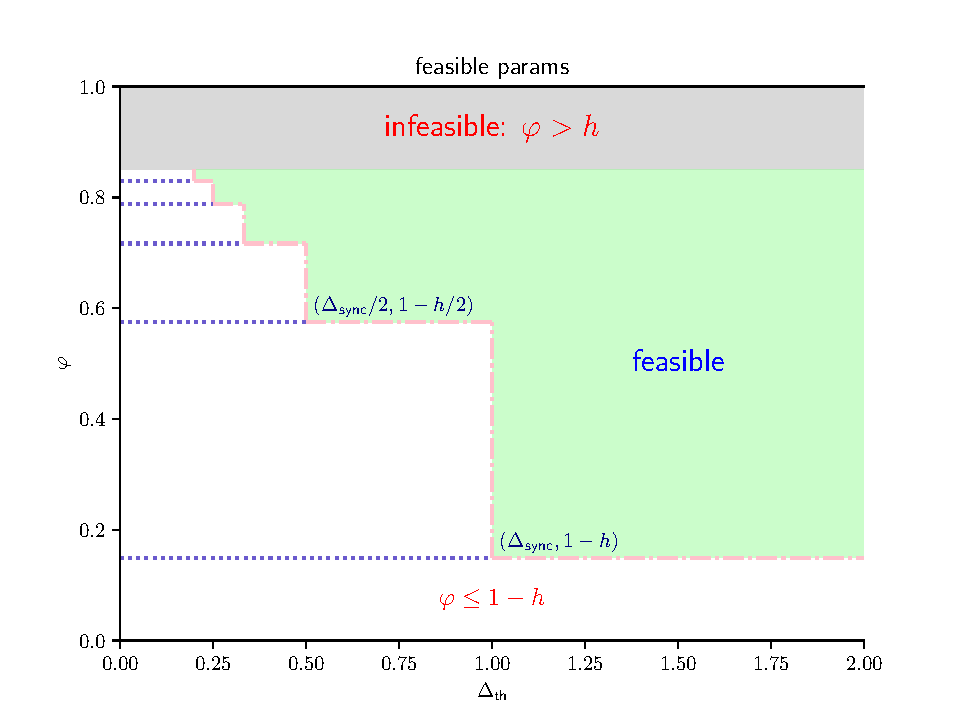
\includegraphics[width=0.7\textwidth]{plots/param.pdf}
    \caption{The set of feasible parameters $(\thtime, \varphi)$ for time-delayed-fairness, where $\synctime=1$ and $h=0.7$. The green shaded area is the feasible region. The boundary lines are $\thtime=1/k$ and $\varphi=1-h/k$ for positive integers $k$. The dashed line is $\varphi=1-h/\lceil 1/\thtime \rceil$. For any point above the dashed line, it is feasible. For any point on or below the dashed line, it is infeasible. }
    \label{fig:params}
\end{figure}

\begin{proof}
    In order to prove the theorem, we need to show that (1) for any paramters in green shaded area of figure \ref{fig:params}, i.e., for any positive integer $k$, when $\thtime>\synctime/k$ and $\varphi>1-h/k$, time-delayed-fairness can be achieved; (2) for any parameters in white area of figure \ref{fig:params}, i.e., (2a) for any positive integer $k$, when $\thtime\leq \synctime/k$ or $\varphi\leq 1-h/k$, time-delayed-fairness cannot be achieved.
\end{proof}

Maybe it works for any rational number $k=\frac{k_1}{k_2}\ge1$. $k_1,k_2$ are coprime positive integers. 


Do we need to exclude bad reports?  No for the case of $k=1$. 


\subsection{Feasibility for $(\thtime>\synctime, \varphi>1-h)$ and Infeasibility for $(\thtime\leq \synctime, \varphi\leq 1-h)$}

}